\chapter{相关原理分析}
\label{xiangguanyuanli}
在本章中,将针对本文涉及的关键技术的原理进行分析和解读,这些关键技术是指导本文工作开展的理论支撑,只有把这些技术原理充分理解后,才能解决设计过程中遇到的难题,才能进行一系列的优化工作。这些技术原理包括,图像表示原理,SIFT算法原理,spark内存技术原理,spark任务调度原理,spark 性能优化原理以及HDFS存储原理。
\section{图像表示原理}
数字图像可以理解为对二维函数$f(x,y)$进行采用和量化后得到的图像,因此,通常用二维矩阵来表示一幅数字图像,矩阵中每一个值代表图像中的一个像素。在现实生活中,我们看到的大多数图像都是彩色的,在彩色图片中,每个像素由R,G,B三个分量组成,每个分量的取值为0~255(0表示最暗,255 表示最亮)。但是在图像处理中大多数用的都是灰度图像,灰度图像是R、G、B三个分量灰度值相同的一种特殊图像。处理中使用灰度图像的原因在于它会使后续的处理时的计算量变得相对很少,并且灰度图像对图像特征的描述与彩色图像没有什么区别,RGB只是从光学的原理上对颜色进行了调配。因此灰度图像仍然能反应整个图像的整体和局部的亮度和色度特征。本文的设计工作就是建立在灰度图像之后,我们将原始的图片都进行了灰度化处理,后续的所有处理都在此基础上进行。

灰度图像的每个像素用一个字节保存,对RGB图像进行灰度化,是对图像中RGB三个分量进行加权平均得到最终的灰度值,加权公式~\ref{jiaquan}所示:
\begin{equation}\label{jiaquan}
 Gray = 0.11B + 0.59G + 0.3R
\end{equation}

理解好基础的图像原理,是Spark下图像基础库SparkImgLib实现的理论指导。
\section{SIFT算法原理}
\label{sec:sift}
在本小节中,将会对SIFT算法进行详细分析,它是Spark下特征提取系统的最核心算法。

SIFT是一种检测并提取图像局部特征的算法,该算法在空间尺度中寻找极值点,并且提取出其位置、尺度、旋转不变量等信息。它的基本特点如下:
\begin{itemize}
\item 局部不变性好。局部特征对旋转,尺度缩放,亮度变化保持不变性,对视角变化,放射变换,噪声也有一定程度的稳定性。
\item 特征信息丰富。算法采用128维向量表示一个特征,基本可以达到准确匹配的效果。
\item 可扩展性强。可以很方便的与其他形式的特征向量进行联合。
\end{itemize}

SIFT算法大体可以划分为5个步骤,分别是高斯塔建立,高斯差分塔建立,极点检测,消除边缘响应,关键点方向的分配和描述,接下来,将会对这几个步骤进行分析:
\begin{compactenum}
\item 高斯塔建立\\图像高斯金子塔是将原始图像不断降阶采用,得到的一系列的大小不一的图像,由大到小,从下到上构成的塔状模型。原图像为金子塔的第一层,每次降采样所得到的新图像为金字塔的一层(每层一张图像),每个金字塔共n 层。为了让尺度体现其连续性,高斯金字塔在简单降采样的基础上加上了高斯滤波。高斯金字塔上一组图像的初始图像(底层图像)是由前一组图像的倒数第三张图像隔点采样得到的。一组高斯金字塔如图~\ref{fig:gausspy}所示:
\begin{figure}[htp]
\centering
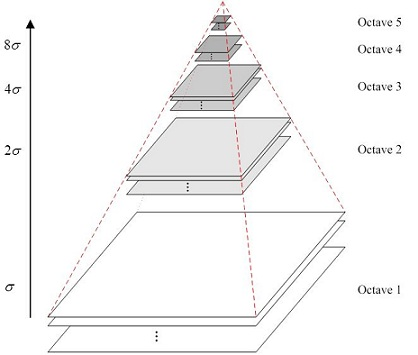
\includegraphics{gausspy}
\caption{图像的一组高斯金字塔}
\label{fig:gausspy}
\end{figure}

高斯金字塔是尺度空间的表示,sift算法是基于尺度空间理论的。尺度空间思想最早是由Iijima\upcite{Iijima}于1962年提出的,后经witkin\upcite{Witkin}和Koenderink\upcite{Koenderink}等人的推广逐渐得到关注,在计算机视觉邻域使用广泛。尺度空间理论的基本思想是:在图像信息处理模型中引入一个被视为尺度的参数,通过连续变化尺度参数获得多尺度下的尺度空间表示序列,对这些序列进行尺度空间主轮廓的提取,并以该主轮廓作为一种特征向量,实现边缘、角点检测和不同分辨率上的特征提取等。尺度理论的数学表达式如公式~\ref{chidu}所示:
\begin{equation}\label{chidu}
L(x,y,\delta)=G(x,y,\delta)*I(x,y)
\end{equation}

其中,*表示卷积运算,G(x,y,$\delta$)为高斯函数,
\begin{equation}\label{gauss}
G(x,y,\delta)=\frac{1}{2\pi{\delta}^2}e^{-\frac{(x-m/2)^2+(y-n/2)^2}{2\delta^2}}
\end{equation}

其中,m和n表示高斯模板的维度,(x,y)代表图像的像素位置,$\delta$是尺度空间因子,值越小表示图像被平滑的越少,相应的尺度也就越小。大尺度对应于图像的概貌特征,小尺度对应于图像的细节特征。

\item 高斯差分金字塔建立\\高斯差分金子塔是在高斯金子塔的基础上的到得,通过将同一组中的相邻层数的高斯图像相减,可以得到高斯差分图像,具体如图~\ref{fig:gaussDog}所示:
\begin{figure}[htp]
\centering
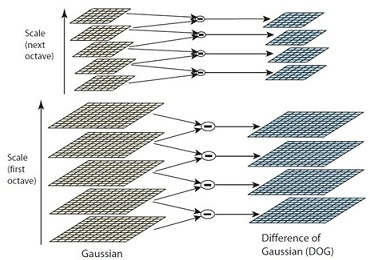
\includegraphics{gaussDog}
\caption{高斯差分金子塔}
\label{fig:gaussDog}
\end{figure}

尺度归一化的高斯拉普拉斯函数${\delta}^2{\nabla}^2{G}$的极大值和极小值同其它的特征提取函数,例如:梯度,Hessian或Harris角特征比较,能够产生最稳定的图像特征。而高斯差分函数(Difference of Gaussian ,简称DOG算子)与尺度归一化的高斯拉普拉斯函数${\delta}^2{\nabla}^2{G}$,它们的关系推导如下:
\begin{equation}\label{dog_1}
\frac{\partial{x}}{\partial{\delta}}=\delta\nabla^2G
\end{equation}

利用差分近似代替微分,则有:
\begin{equation}\label{dog_2}
\delta\nabla^2G=\frac{\partial{x}}{\partial{\delta}}\approx\frac{G(x,y,k\delta)-G(x,y,\delta)}{k\delta-\delta}
\end{equation}

因此就有:
\begin{equation}\label{dog_3}
G(x,y,k\delta)-G(x,y,\delta)\approx(k-1)\delta^2\nabla^2G
\end{equation}

其中k-1是常数,并不影响极值点的位置求取,两者极值关系如图~\ref{fig:py_dog}所示,其中横坐标为0处,最下方的曲线为高斯差分算子,上方为高斯拉普拉斯算子:
\begin{figure}[htp]
\centering
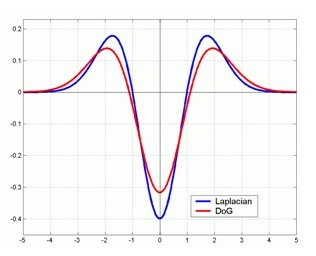
\includegraphics{py_dog}
\caption{高斯拉普拉斯和高斯差分极值关系对比}
\label{fig:py_dog}
\end{figure}

当使用高斯差分算子代替拉普拉斯算子进行极值检测,公式如下所示:
\begin{equation}\label{dog_detect}
D(x,y,\delta)=\Bigl(G(x,y,k\delta)-G(x,y,\delta)\Bigr)*I(x,y)=L(x,y,k\delta)-L(x,y,\delta)
\end{equation}

在实际计算时,使用高斯金字塔每组中相邻上下两层图像相减,得到高斯差分图像,然后在差分图像上进行极点检测。
\item 极点检测\\关键点是由DOG空间的局部极值点组成的,关键点的初步探查是通过同一组内各DoG相邻两层图像之间比较完成的。为了寻找DoG函数的极值点,每一个像素点要和它所有的相邻点比较,看其是否比它的图像域和尺度域的相邻点大或者小。如图3.4所示,中间的检测点和它同尺度的8个相邻点和上下相邻尺度对应的9×2个点共26个点比较,以确保在尺度空间和二维图像空间都检测到极值点。具体如图~\ref{fig:pole_detect}所示:
\begin{figure}[htp]
\centering
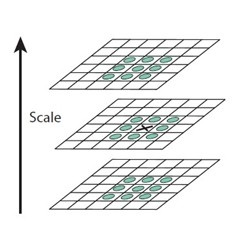
\includegraphics{pole_detect}
\caption{高斯差分图像上的极点检测}
\label{fig:pole_detect}
\end{figure}

\item 关键点精确定位\\离散空间的极值点并不是真正的极值点,图~\ref{fig:keypoint_detect}显示了二维函数离散空间得到的极值点与连续空间极值点的差别。利用已知的离散空间点插值得到的连续空间极值点的方法叫做子像素插值(Sub-pixel Interpolation)。
\begin{figure}[htp]
\centering
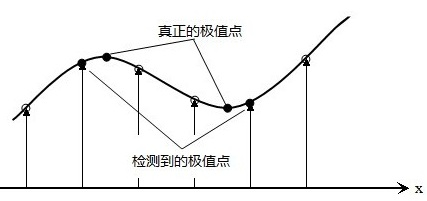
\includegraphics{keypoint_detect}
\caption{离散空间与连续空间极值点的差别}
\label{fig:keypoint_detect}
\end{figure}

为了提高关键点的稳定性,需要对尺度空间DoG函数进行曲线拟合。利用DoG函数在尺度空间的Taylor展开式(拟合函数)如公式~\ref{Tayor},其中$X={(x,y,\delta)^T}$代表相对插值中心的偏移量,当它在任一维度上的偏移量大于0.5时(即x或y或$\delta$),意味着插值中心已经偏移到它的邻近点上,所以必须改变当前关键点的位置,同时在新的位置上反复插值直到收敛,但是此过程有可能超出设定测迭代次数或者图像边界范围,那么这样的点就应该被删除掉,在Lowe的论文中,迭代的上限为5。另外,${|D(x)|}$的值过小会受到噪声影响而变得不稳定,因此该值小于某个阈值的极值点也要删除,在Lowe论文中,使用阈值的大小为0.03。
\begin{equation}\label{Tayor}
D(X)=D+\frac{\partial{D}^T}{\partial{X}}X+\frac{1}{2}X^T\frac{\partial^2{D}}{\partial{X}^2}X
\end{equation}

\item 关键点方向分配和描述\\为了使描述符具有旋转不变性,需要利用图像的局部特征为给每一个关键点分配一个基准方向。使用图像梯度的方法求取局部结构的稳定方向。对于在DOG金字塔中检测出的关键点点,采集其所在高斯金字塔图像3σ邻域窗口内像素的梯度和方向分布特征。梯度的模值和方向如下:
\begin{equation}\label{mozhi}
m(x,y)=\sqrt{L(x+1,y)-{L(x-1,y)}^2+L(x,y+1)-{L(x,y-1)}^2}
\end{equation}
\begin{equation}\label{fangxiang}
\theta(x,y)=\tan^{-1}\Bigl({\frac{L(x,y+1)-L(x,y-1)}{L(x+1,y-L(x-1,y)}}\Bigr)
\end{equation}
\end{compactenum}

其中,L为关键点所在尺度的空间值,邻域窗口半径为3*1.5${\delta}$。

在完成关键点的梯度计算后,使用直方图统计邻域内像素的梯度和方向。梯度直方图将0~360度的方向范围分为36个柱(bins),其中每柱10度。如图~\ref{fig:direct_histogram}所示,直方图的峰值方向代表了关键点的主方向,(为简化,图中只画了八个方向的直方图)。方向直方图的峰值则代表了该特征点处邻域梯度的方向,以直方图中最大值作为该关键点的主方向。为了增强匹配的鲁棒性,只保留峰值大于主方向峰值80%的方向作为该关键点的辅方向。因此,对于同一梯度值的多个峰值的关键点位置,在相同位置和尺度将会有多个关键点被创建但方向不同。仅有15%的关键点被赋予多个方向,但可以明显的提高关键点匹配的稳定性。
\begin{figure}[htp]
\centering
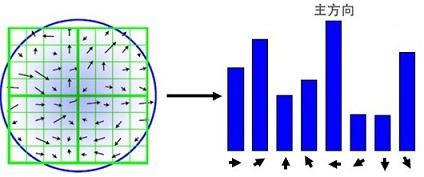
\includegraphics{direct_histogram}
\caption{关键点方向直方图}
\label{fig:direct_histogram}
\end{figure}

在关键点方向被确定之后,我们需要给这些关键点建立一个定量的描述,该描述子不仅包括关键点的信息,也包含关键点周围对其有贡献的像素点,并且描述符应该有较高的独特性,以便于提高特征点正确匹配的概率。SIFT算法中通过一组向量将关键点的特征描述出来,SIFT描述子是关键点邻域高斯图像梯度统计结果的一种表示。通过对关键点周围图像区域分块,计算块内梯度直方图,生成具有独特性的向量,这个向量是该区域图像信息的一种抽象,具有唯一性。

Lowe在论文中建议使用在关键点尺度空间内4*4的窗口中计算的8个方向的梯度信息,共4*4*8=128维向量表征,具体表示步骤如下:
\begin{itemize}
\item 确定计算描述子所需的图像区域
\item 将坐标轴旋转为关键点的方向,以确保旋转不变性
\item 将邻域内的采样点分配到对应的子区域内,将子区域内的梯度值分配到8个方向上,计算其权值
\item 插值计算每个种子点八个方向的梯度
\item 描述子向量门限
\item 按特征点的尺度对特征描述向量进行排序
\end{itemize}

至此,SIFT特征描述向量生成完毕。

在上述5个步骤中,构建高斯金字塔和极点检测是最为耗时的两个。构建高斯金字塔时需要对每张图片进行高斯滤波,高斯滤波是一个时间复杂度为O(N3) 的操作,这里的N与图像大小成正比。图~\ref{fig:gausspy}中仅显示了一组金字塔,而SIFT算法往往需要构建多组金字塔,使得构建高斯金字塔的时间复杂度达到O(O*I*N3),其中O为高斯塔的组数,I为高斯塔的层数。极点检测则是在整个金字塔组上进行的,相当于在一个维度为4的空间(组,层,长,宽)中搜索极值点,它的时间复杂度为O(O*I*N2)。SIFT算法流程中既包含高斯滤波和图像缩放等通用性较强的操作,也含有构建高斯(查分)金字塔、极点检测、消除边缘响应等通用性较差的操作。它的空间复杂度和时间复杂度都比较高,当有海量的图片需要进行特征提取时,占用内存较多,所需的处理时间也会很长。这也是我们使用Spark去加速SIFT算法的原因。

只有充分理解SIFT算法原理之后,才能比较好的在Spark上实现大规模特征提取工作。

\section{Spark核心技术原理}
在这一小节中,将会对Spark中三个核心技术原理进行分析,它们分别是内存编程原理,任务调度原理,性能优化。这三个技术在本文的设计起非常重要的地位,只有将这些技术理解透彻后,才能自如的解决开发过程中遇到的问题。
\subsection{Spark内存编程原理}
Spark区别于其他的大数据处理框架,比如Hadoop\upcite{Hadoop},在于它是一个内存计算的大数据处理框架,它可以将处理的中间结果保存在内存中,后续的计算可以在此基础上直接运行,提升了执行的效率。那么,这么多的数据保存在内存中,这就必须基于分布式内存的数据结构抽象,让开发人员基于该数据结构进行操作,只要操作这些数据,它们就是位于集群的内存中的。上面说的内存抽象数据结构就是RDD(Resilient Distributed Dataset弹性分布式数据集),RDD是Spark最核心的概念,接下来将从RDD的底层实现原理,RDD的操作类型,RDD的缓存原理,RDD 的依赖关系和DAG的生成这几方面分析RDD。
\subsubsection{RDD的底层实现原理}
RDD的基本单元是分区(Partition),一个RDD由多个分区组成,每个分区都会被逻辑映射成一个Block,一个Block会被一个Task执行,这些Block由BlockManager管理,BlockManager负责管理这些Block在集群内的分布。整个过程如图~\ref{fig:blockmanager}所示:
\begin{figure}[htp]
\centering
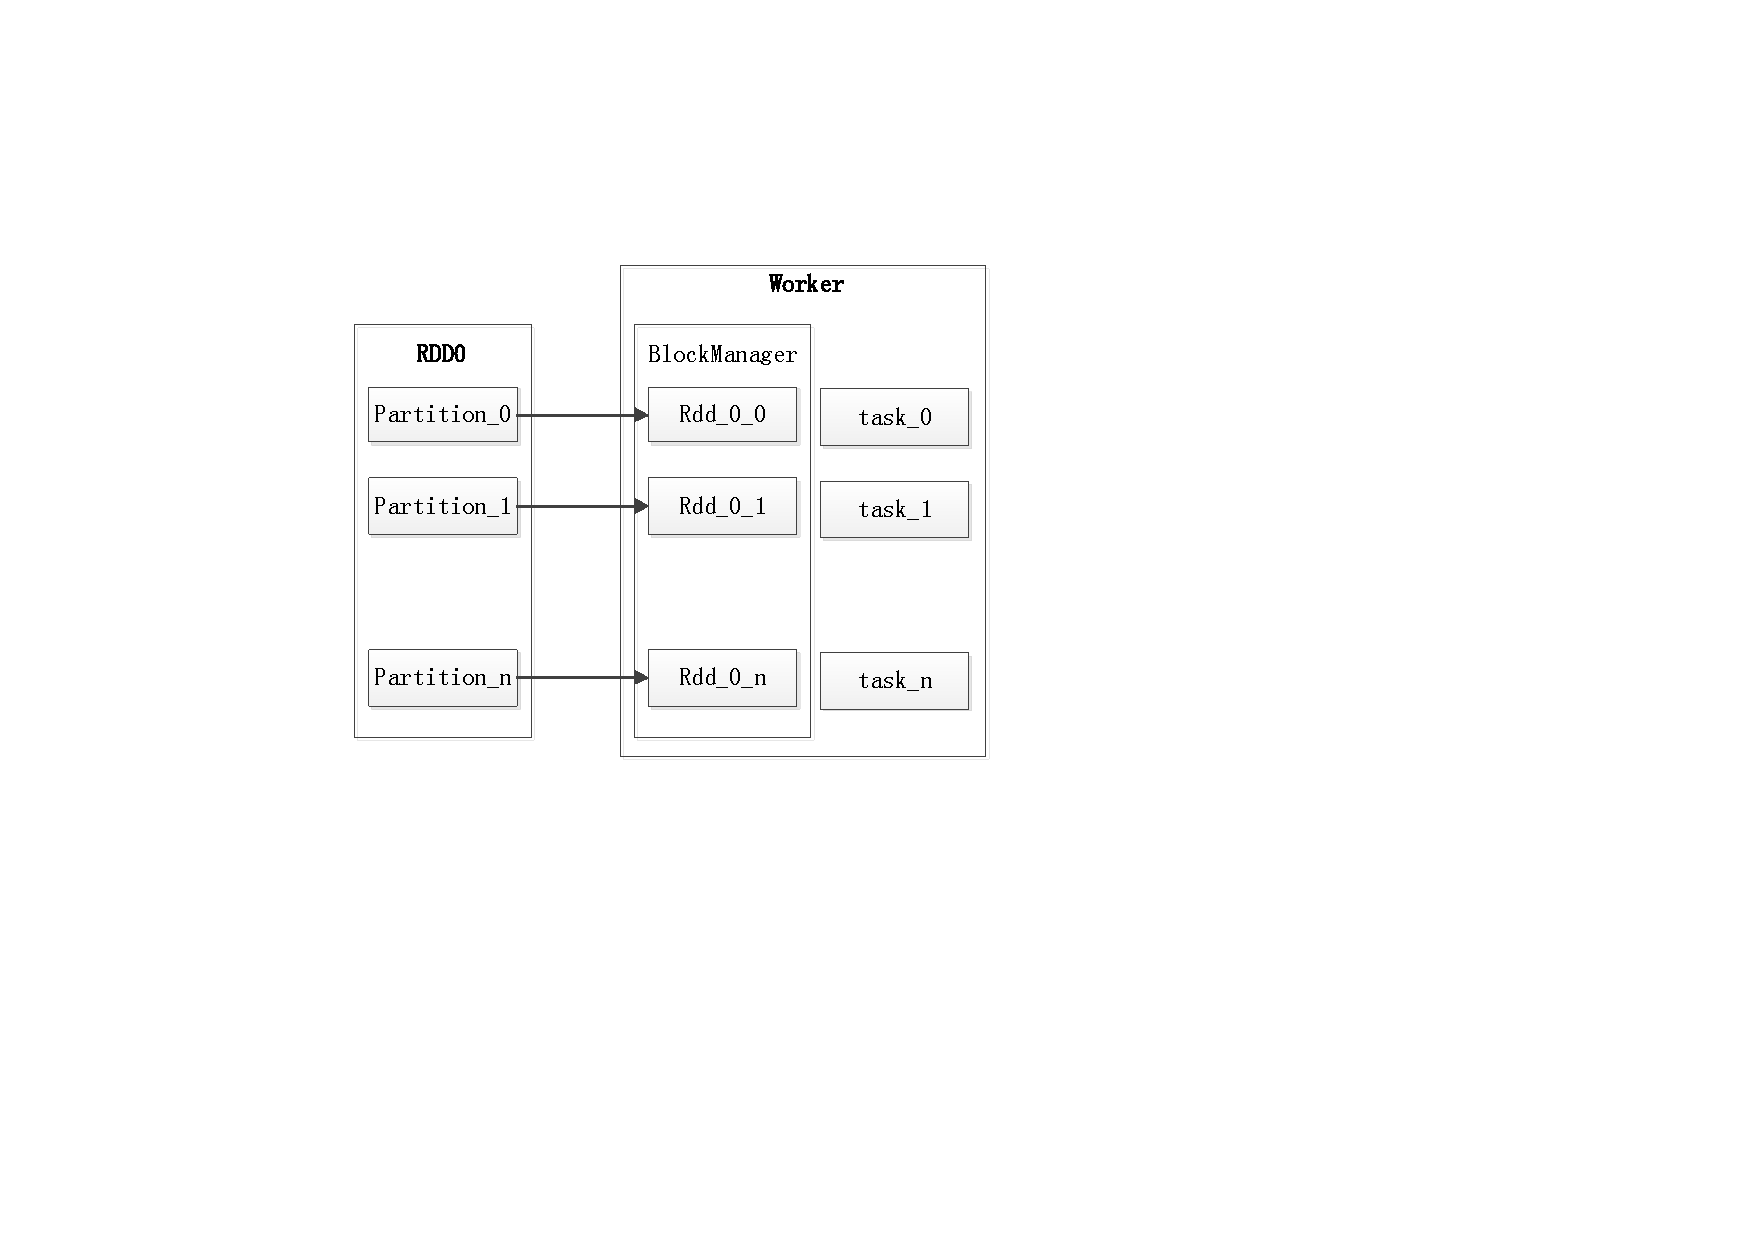
\includegraphics{blockmanager}
\caption{RDD Partition的存储和计算模型}
\label{fig:blockmanager}
\end{figure}

\subsubsection{RDD的操作类型}
RDD提供的操作可以分为两种类型,分别是transformtion(转换)和action(动作),表\ref{tab:trans}和表\ref{tab:action}分别列出了常用的转换操作和动作操作。所有的转换操作都是惰性的,被调用时,它们不会直接计算结果,它们只是记住上一个转换动作,当一个动作操作被调用时,这些转换操作才会被执行。这种设计会让Spark运行得更加高效率,因为可能在动作操作时,被操作的数据集会变得比较小。
\begin{table}[h] %开始一个表格environment,表格的位置是h,here。
\caption{RDD转换操作} %显示表格的标题
\centering
\label{tab:trans}
\begin{tabular}{p{6cm}|p{8cm}} %设置了每一列的宽度,强制转换。
\hline
\hline
转换  & 含义 \\ %用&来分隔单元格的内容 \\表示进入下一行
\hline %画一个横线,下面的就都是一样了,这里一共有4行内容
map(func)  & 返回一个新的分布式的数据集,该数据集有每一个输入元素经过func函数转换后组成\\
\hline
filter(func)  & 返回一个新的数据集,该数据集经过func函数计算后返回值为true的输入元素组成\\
\hline
flatMap(func)  & 类似于Map,但是每一个输入元素可以被映射为0个或者是多个输出元素\\
\hline
mapPartitions(func) & 类型于map,但是独立在RDD的每一个分片上运行,因此func的类型必须是Iterator[T]=>Iterator[U]\\
\hline
mapPartitionWithSplit(func) & 类似于mapPartitions,但是func带有一个整型参数表示分片的索引值,func的函数类型为(Int,Iterator[T])=>Iterator[U]\\
\hline
sample(withReplacement,fraction,seed) & 根据fraction指定比例对数据进行采用\\
\hline
union(otherDataset) & 返回一个新的数据集,新数据集是由源数据集和参数数据集联合而成的\\
\hline
distinct(numTasks) & 返回一个包含源数据集中所有不重复的元素的新的数据集\\
\hline
\hline
\end{tabular}
\end{table}

\begin{table}[h] %开始一个表格environment,表格的位置是h,here。
\caption{RDD动作操作} %显示表格的标题
\centering
\label{tab:action}
\begin{tabular}{p{6cm}|p{8cm}} %设置了每一列的宽度,强制转换。
\hline
\hline
动作  & 含义 \\ %用&来分隔单元格的内容 \\表示进入下一行
\hline %画一个横线,下面的就都是一样了,这里一共有4行内容
reduce(func)  & 通过函数func聚集数据集中的所有元素\\
\hline
collect()  & 在驱动程序中,以数组的形式返回数据集中的所有元素。通常在使用filter或者其他操作返回一个足够小的数据子集后再使用比较有用\\
\hline
count()  & 返回数据集的个数\\
\hline
first() & 返回数据集的第一个元素\\
\hline
take(n) & 返回一个由数据集的前n个元素组成的数组\\
\hline
takeSample(withReplacement,num,seed) & 返回一个数组,该数组由从数据集中随机采用的num个元素组成\\
\hline
saveAsTextFile(path) & 将数据集的元素以textFile的形式保存到本地文件系统,HDFS或者任何Hadoop支持的文件系统\\
\hline
saveAsSequenceFile(path) & 将数据集的元素以Hadoop sequencefile的格式保存到指定目录下,可以是本地系统,HDFS或者任何Hadoop支持的文件系统\\
\hline
countByKey() & 对(K,V)类型的RDD有效,返回一个(K,Int)对的map,表示每一个key的元素个数\\
\hline
foreach(func) & 在数据集的每一个元素上,运行函数func进行更新\\
\hline
\hline
\end{tabular}
\end{table}

\subsubsection{RDD的缓存原理}
spark速度非常快的原因之一,就是在不同操作中内存中持久化(或缓存)一个数据集。当持久化一个RDD后,每一个节点都将会把计算分片的结果保存在内存中,后续的其他操作可以直接使用该结果,这就使得后续的动作变得十分迅速。

通过persist()或cache()方法可以标识一个要被持久化的RDD,一旦首次被触发后,该RDD将会被保留在计算节点的内存中并重用。persist()和cache()的实现如下:
\begin{lstlisting}[language=Java,numbers=none,frame=none]
/**Persist this RDD with the default storage level('MEMORY_ONLY').*/
def persist(): this.type = persist(StorageLevel.MEMORY_ONLY)
/**Persist this RDD with the default storage level('MEMORY_ONLY').*/
def cache(): this.type = persist()
\end{lstlisting}

假设首先进行了RDD0$\rightarrow$RDD1$\rightarrow$RDD2的计算作业,如果RDD1已经被缓存在内存中,那么后续在进行RDD0$\rightarrow$RDD1$\rightarrow$RDD3的计算作业时,就不需要从头开始,直接从RDD1往下执行作业即可,因此计算速度得到了很大的提升,具体过程如下图\ref{fig:rdd_cache}所示:
\begin{figure}[htp]
\centering
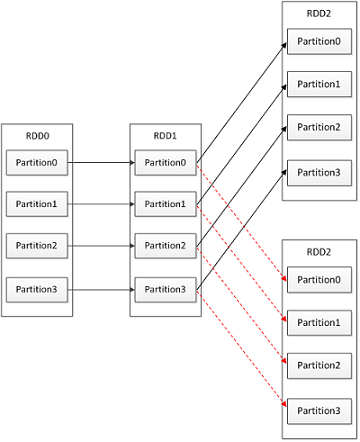
\includegraphics{rdd_cache}
\caption{RDD 缓存加速原理}
\label{fig:rdd_cache}
\end{figure}

缓存的rdd有可能会丢失,或者因为内存不足而删除,但是rdd有完整的容错机制,保证在rdd丢失或者删除的情况下计算依然可以正确执行。
\subsubsection{RDD的依赖关系和DAG的生成}
一个Spark应用中,不同的RDD间存在依赖关系,依赖关系分为窄依赖(narrow dependency)和宽依赖(wide dependency),窄依赖和宽依赖的定义如下:
\begin{itemize}
\item 窄依赖,窄依赖是指父RDD的每个分区只被子RDD的一个分区所使用,如图\ref{fig:dependency}左边部分显示
\item 宽依赖,宽依赖是指父RDD的每个分区都可能被多个子RDD分区所使用,如图\ref{fig:dependency}右边部分显示
\end{itemize}
\begin{figure}[htp]
\centering
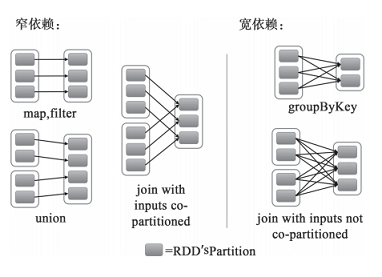
\includegraphics{dependency}
\caption{RDD窄依赖和宽依赖对比}
\label{fig:dependency}
\end{figure}
在Spark应用开发中,RDD会经过很多转换操作,每个转换操作都会生成一个新的RDD,这些转换操作最后会形成一个有向图(Directed Acyclic Graph,简称DAG)。这个DAG记录着RDD间的依赖关系,借助这些依赖关系,能保证一个RDD被计算前,所有它所依赖的parent RDD都已经完成了计算。同时Spark 也是整个DAG根据依赖关系的不同划分为不同的阶段(stage),一个stage中包含的一组并行执行的任务。划分stage的依据是,rdd间是窄依赖关系的划分到一个stage中,rdd间是宽依赖的划分到不同的stage中。一个stage中可以并行执行,不同stage 间顺行执行。
\subsection{Spark任务调度原理}
Spark任务调度框架主要由三个模块支撑起,它们分别是DAGScheduler,SchedulerBackend及TaskScheduler。首先DAGScheduler分析用户提交的应用,根据依赖关系建立DAG,然后将DAG 划分为不同的Stage,而stage中包含所要执行的tasks。SchedulerBackend负责整个集群交互,收集可用的资源信息,然后将这些信息上报TaskScheduler。TaskScheduler将从SchedulerBackend获取到的资源信息以及从DAGScheduler生成的tasks进行一个资源的分配,将tasks分配的合适的资源上面。整个流程如图\ref{fig:schedulerfw}所示:
\begin{figure}[htp]
\centering
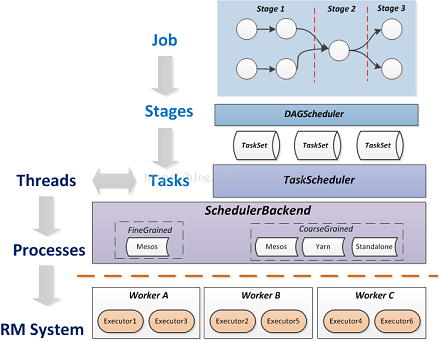
\includegraphics{schedulerfw}
\caption{Spark任务调度框架}
\label{fig:schedulerfw}
\end{figure}
\subsubsection{DAGScheduler}
DAGScheduler面向stage的调度(stage-oriented scheduling)的高级调度器,将job根据类型划分为不同的stage(划分的依据是依赖关系为窄依赖的属于一个stage,依赖关系为宽依赖的RDD属于不同的stage)为每个job 的不同stage 计算DAG,跟踪哪些RDD和stage被物化并且发现运行job的最小的调度策略,然后并在每一个stage 内产生一系列的task 并封装为taskset, 结合当前的缓存情况来决定每个Task的最佳位置(任务在数据所在的节点上运行),以taskset 为单位提交(submitTasks) 给TaskScheduler。
\subsubsection{SchedulerBackend}
SchedulerBackend负责与Cluster Manager交互,取得该Application分配到的资源,并且将这些资源传给TaskScheduler,由TaskScheduler为Task最终分配计算资源。在不同的集群模式下,SchedulerBackend的实现是不一样的,实现可以分为细粒度和粗粒度两种。分为细粒度和粗粒度两种。细粒度只有Mesos(mesos有粗细两种粒度的使用方式)实现了,粗粒度的实现者有yarn,mesos,standalone。拿standalone模式来说粗粒度,每台物理机器是一个worker,worker一共可以使用多少cpu和内存,启动时候可以指定每个worker起几个executor,即进程,每个executor的cpu和内存是多少。粗粒度与细粒度的主要区别,就是粗粒度是进程long-running 的,计算线程可以调到executor上跑,但executor的cpu和内存更容易浪费。细粒度的话,可以存在复用,可以实现抢占等等更加苛刻但促进资源利用率的事情。这俩概念还是AMPLab论文里最先提出来并在Mesos里实现的。AMPLab在资源使用粒度甚至任务分配最优的这块领域有不少论文,包括Mesos的DRF算法、Sparrow调度器等。所以standalone模式下,根据RDD的partition数,以及每个task需要的cpu 数,可以很容易计算每台物理机器的负载量、资源的消耗情况、甚至知道TaskSet要分几批才能跑完一个stage。
\subsubsection{TaskScheduler}
TaskScheduler负责Application的不同Job间的调度,在Task执行失败时启动重试机制。TaskScheduler里会对已经提交的tasks进行一次优先级排序,这个排序策略目前有两种:FIFO(First In First Out,先进先出)或FAIR(公平调度),默认调度策略是FIFO。通过排序,会得到一份待运行的tasks,然后就把从schedulerBackend交过来的worker资源信息合理分配给这些tasks。分配前,为了避免每次都是前几个worker被分到tasks,所以先对WorkerOffer列表进行一次随机洗牌。接下来就是遍历tasks,看workers的资源“够不够”,“符不符合”task,如果符合的话task就被正式launch起来。
\subsection{Spark性能优化原理}
在本小节中,将介绍Spark的性能优化原理,因为Spark是处理大数据的框架,因此性能优化是非常有必要的。接下来将从几个方面分析spark的性能问题
\subsubsection{调度和分区优化}
在spark应用程序中,会经常使用fiter算子进行数据过滤,而频繁的过滤或者过滤的数据量过大就会造成大量小分区,由于spark是每个数据分区都会分配一个任务执行,如果任务过多,就会造成线程切换开销很大,很多任务等待执行,并行度实际上不高。面对这种情况,我们可以采用RDD中的重分区函数进行数据的紧缩,减少分区数,将小分区合并成大分区。具体可以通过coalesce函数进行,函数定义如下:
\begin{lstlisting}[language=Java,numbers=none,frame=none]
def coalesce(numPartitions: Int, shuffle: Boolean = false)(implicit ord: Ordering[T] = null): RDD[T]
\end{lstlisting}

该函数会返回一个含有numPartitions数量个分区的新的RDD,即将整个RDD重分区。

使用这个函数会出现一个问题,比如将1000个分区的RDD重分区为一个分区,就会造成数据过于集中,完成无法开掘集群并行计算的能力。在这种情况下,可以将coalsesce 函数参数shuffle 设置为true,由于shuffle 可以分隔shuffle,这就保证了上游的任务仍是1000个,否则两个上下游的任务合并为一个stage 计算,这个stage就会在一个分区上进行并行计算。

除了将分区收缩,在某些情况下,可能会对原来的分区进行扩充,将分区数量增加,以利用并行计算能力。在这个过程中,默认使用的是Hash分区器进行重分区。

在分区优化问题中,还有一个倾斜(skew)的问题。倾斜是一个大数据处理中一个非常重要的问题,可以分为数据倾斜和任务倾斜,数据倾斜的结果就会造成任务倾斜,在个别分区上,任务的执行时间过长。
\begin{compactenum}
\item 数据倾斜\\产生数据倾斜的原因大致有这几种:
\begin{itemize}
\item key数据分布不均匀,因为spark中默认是按照Hash方式进行分区,如果某个key的数据特别多,就会造成分到某个key上的数据特别多,最后造成某个分区的数据特别多,也就出现了数据倾斜。
\item 结构化数据表设计问题
\item 某些SQL语句产生数据倾斜
\end{itemize}

\item 任务倾斜\\产生任务倾斜的原因较为隐蔽,有可能是服务器架构的原因,有可能是JVM的原因,有可能是线程池的原因,也有可能是业务本省的原因。比如在本文设计中就发现,即使是两个任务的处理数据的总大小一样,但是仍然会产生任务倾斜,这和处理问题的具体场景有关系,在SIFT算法中,算法的时间复杂度和图片的尺寸大小有关系的。
\end{compactenum}

\subsubsection{内存存储优化}
因为spark是内存计算的大数据处理框架,因此内存存储优化也是十分重要的内容。内存调优过程中,有三个方向值得考虑,分别是JVM调优,OOM问题调优及磁盘临时目录空间优化。
\begin{compactenum}
\item JVM调优\\不同的JAVA对象都有一个对象头,这些信息有时候比数据本身的信息还要大,比如只有一个Int属性的对象。还有一些链式结构,它们会包含一些指针信息。因此在开发的过程要选好数据类型和数据结构,尽量减少一些链式结构的使用;减少对象的嵌套;可以考虑使用数字ID或者是枚举对象,而不是字符串作为key的关键数据。
\item OMM问题调优\\在spark开发过程中,内存溢出(OutOfMemoryError)是一个经常会遇到的问题,发生内存溢出的原因是Java虚拟机创建的对象太多,在进行垃圾回收时,虚拟机分配的堆空间已经用满了,与heap space有关。解决这类问题有两种思路,一种是减少App的内存占用空间消耗,另一种是增大内存资源的供应。具体设计时,可以查看程序中是否有循环创建对象的地方,程序中应该减少这种代码的存在,或者可以调整JVM中的Xmx(最大堆)和Xms(最小堆)参数的大小。另外,还要查看在做shuffle类操作符时是否创建的Hash表过大,在这种情况下,可以通过增加任务数,即分区数来提升并行度,减少每个任务的输入数据,减少内存占用来解决问题。
\end{compactenum}

\subsubsection{磁盘临时目录空间优化}
Spark在进行shuffle的过程中,中间结果会写到spark在磁盘的临时目录中,如果临时目录过小的话,会造成No Space left on device异常,在这种情况下可以配置多个盘块来扩展Spark的磁盘临时目录,让更多的数据可以写到磁盘,加快I/O速度。
\subsubsection{网络传输优化}
Spark是大数据处理框架,因此集群中数据传输也是影响应用性能的重要因素。如果可以减少数据传输的次数或者是传输的大小,可能会极大的提高应用的性能。下面将分析spark中数据传输优化的场景。
\begin{compactenum}
\item 大局部变量的传输\\默认情况下,算子函数内,如果使用了外部变量,那么会将这个变量的拷贝到执行这个函数的每一个task中,如果这个变量十分大,比如是一个大数组,而且执行的任务又特别多,那么网络的传输耗费就会特别大。下面就是一个例子的展示,其中factor就是一个变量,它在map任务中被使用:
\begin{lstlisting}[language=Java,numbers=none,frame=none]
val factor = 3
rdd.map(num => num*factor)
\end{lstlisting}

面对这种情况,可以使用Spark的Brodcast(广播)变量对数据传输进行优化,通过Brocast变量将用到的大数据量数据进行广播发送,可以提升整体速度。Broadcast主广播的变量是只读的,并且在每个节点上只会有一份副本,而不会为每个task都拷贝一个副本。因此就减少了变量到各个节点的网络传输消耗,以及在各个节点上的内存消耗。
\item 大结果收集\\在spark的开发中,会经常用到collect操作,collect操作将各个分区的结果收集到一个数组,返回到driver。如图\ref{fig:collect}如果收集的结果过大,就会拖慢应用的执行时间,甚至造成内存溢出。
\begin{figure}[htp]
\centering
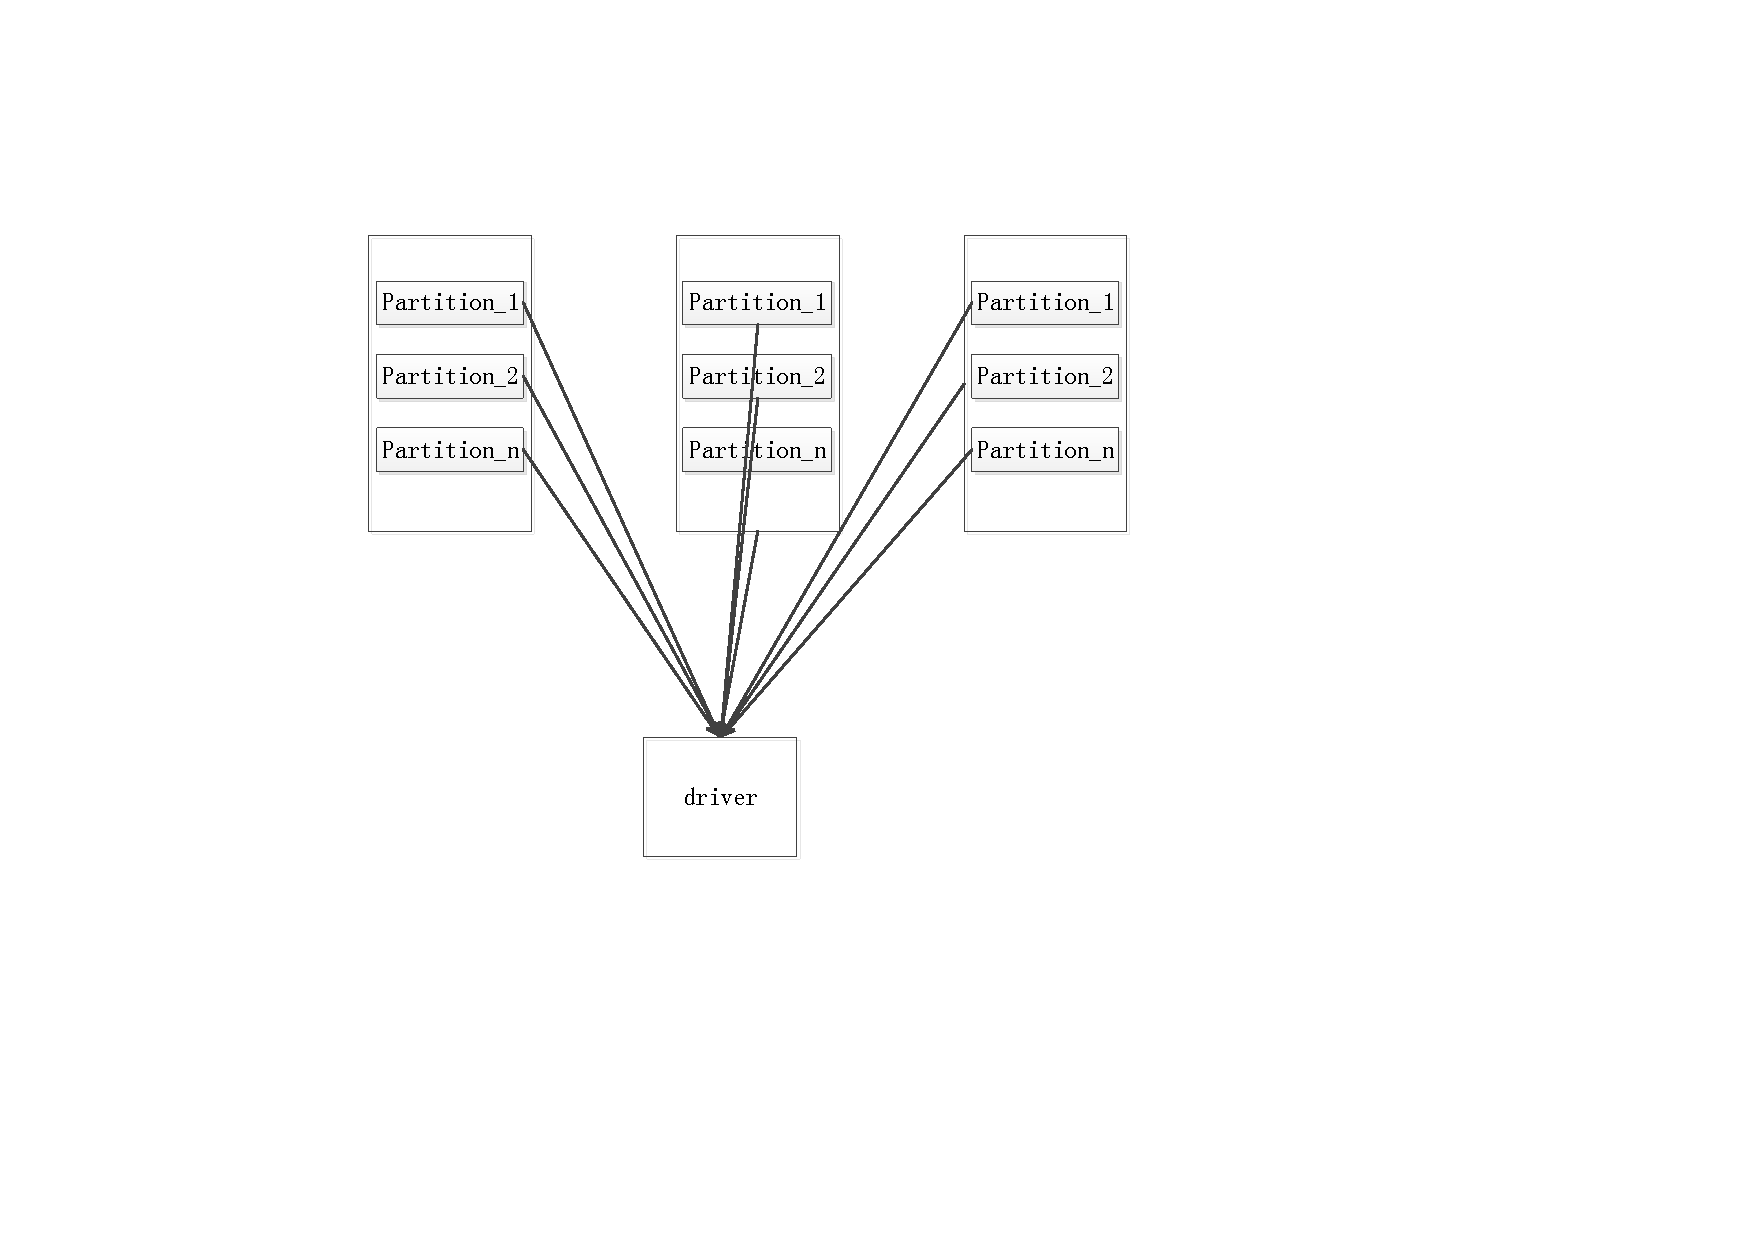
\includegraphics{collect}
\caption{collect操作收集所有分区}
\label{fig:collect}
\end{figure}
面对这种情况,如果收集的结果过大,可以将数据分布式的存储在HDFS或者其他的分布式持久化层上,这样可以减少单机数据的I/O开销和单机内存的存储压力。
%%\subsubsection{序列化与压缩}
\end{compactenum}
\section{分布式存储原理}

\section{GPU特征提取原理}

\section{本章小结}
本章分析了本文工作的一些技术原理,首先分析SIFT算法原理,主要针对SIFT算法的5个主要步骤进行分析,分析其数学原理及作用,然后讨论了算法的时间复杂性。接着介绍了作为本文设计的计算引擎Spark,主要涉及了Spark核心技术原理,主要包括Spark的内存编程原理,任务调度原理,性能优化原理。最后介绍了本文设计中作为存储层的分布式文件系统HDFS的一些核心原理。最后,介绍了作为本文设计的比较的GPU特征提取原理。


